\documentclass[12pt]{article}
\usepackage[utf8]{inputenc}
\usepackage{amsmath}
\usepackage{amsfonts}
\usepackage{amssymb}
\usepackage{graphicx}
\usepackage{tikz}
\usetikzlibrary{positioning}
\usepackage{geometry}
\usepackage{listings}
\usepackage{xcolor}
\usepackage{hyperref}

\geometry{margin=1in}

\title{Audio Processing Pipeline: STFT and Mel-Spectrogram}
\author{Audio Signal Processing Guide}
\date{\today}

\begin{document}

\maketitle

\section{The Complete Audio Processing Pipeline}

The audio processing pipeline transforms raw audio into a format suitable for machine learning models, particularly for emotion recognition in music.

\subsection{Pipeline Overview}

\begin{center}
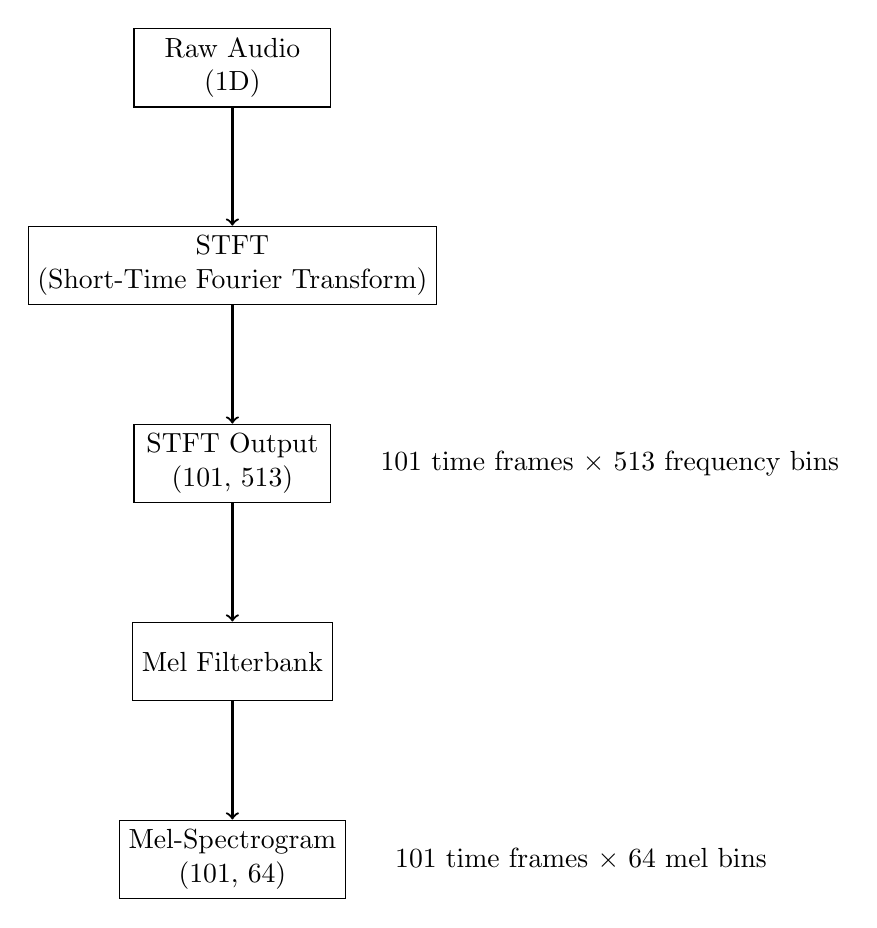
\begin{tikzpicture}[
    node distance=1.5cm,
    box/.style={rectangle, draw, minimum width=2.5cm, minimum height=1cm, align=center},
    arrow/.style={->, thick}
]

% Nodes
\node[box] (raw) {Raw Audio\\(1D)};
\node[box, below=of raw] (stft) {STFT\\(Short-Time Fourier Transform)};
\node[box, below=of stft] (stft_out) {STFT Output\\(101, 513)};
\node[box, below=of stft_out] (mel) {Mel Filterbank};
\node[box, below=of mel] (mel_out) {Mel-Spectrogram\\(101, 64)};

% Arrows
\draw[arrow] (raw) -- (stft);
\draw[arrow] (stft) -- (stft_out);
\draw[arrow] (stft_out) -- (mel);
\draw[arrow] (mel) -- (mel_out);

% Labels
\node[right=0.5cm of stft_out] {101 time frames $\times$ 513 frequency bins};
\node[right=0.5cm of mel_out] {101 time frames $\times$ 64 mel bins};

\end{tikzpicture}
\end{center}

\subsection{Detailed Pipeline Steps}

\begin{enumerate}
    \item \textbf{Raw Audio (1D)}: Input audio signal (e.g., 1 second = 32,000 samples)
    \item \textbf{STFT}: Breaks audio into time-frequency components
    \item \textbf{STFT Output}: Creates 2D matrix of frequency content over time (101 time frames)
    \item \textbf{Mel Filterbank}: Compresses frequency dimension using perceptual scaling
    \item \textbf{Mel-Spectrogram}: Final 2D representation for machine learning (101 time frames)
\end{enumerate}

\section{What STFT Does}

\subsection{Core Function}
STFT (Short-Time Fourier Transform) breaks down an audio signal into \textbf{time-frequency components} by:

\begin{enumerate}
    \item \textbf{Sliding a window} across the audio signal
    \item \textbf{Taking FFT} of each windowed segment
    \item \textbf{Creating a 2D representation}: Time (x-axis) $\times$ Frequency (y-axis)
\end{enumerate}

\subsection{Simple Analogy}
Think of STFT like taking \textbf{snapshots} of the audio every 0.01 seconds, where each snapshot shows \textbf{what frequencies are present at that moment}.

\subsection{Mathematical Parameters}
\begin{align}
\text{Time resolution} &= \frac{\text{hop\_size}}{\text{sample\_rate}} = \frac{320}{32000} = 0.01 \text{ seconds} \\
\text{Number of frames} &= 1 + \frac{\text{signal\_length} + \text{pad} - \text{window\_size}}{\text{hop\_size}} \\
&= 1 + \frac{32000 + 1024 - 1024}{320} = 1 + 100 = 101 \text{ frames} \\
\text{Frequency bins} &= \frac{\text{n\_fft}}{2} + 1 = \frac{1024}{2} + 1 = 513 \text{ bins}
\end{align}

\subsection{Input $\rightarrow$ Output}
\begin{center}
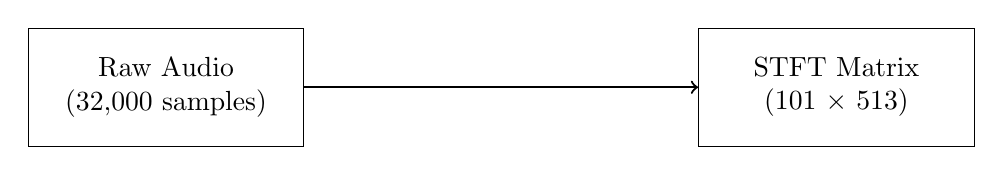
\begin{tikzpicture}[
    node distance=5cm,
    box/.style={rectangle, draw, minimum width=3.5cm, minimum height=1.5cm, align=center},
    arrow/.style={->, thick}
]

\node[box] (input) {Raw Audio\\(32,000 samples)};
\node[box, right=of input] (output) {STFT Matrix\\(101 $\times$ 513)};

\draw[arrow] (input) -- (output);

\end{tikzpicture}
\end{center}

\subsection{Why STFT is Useful}
\begin{itemize}
    \item \textbf{Captures temporal changes} in frequency content
    \item \textbf{Reveals patterns} like beats, notes, and emotional transitions
    \item \textbf{Creates image-like data} that CNNs can process
    \item \textbf{Enables analysis} of when specific frequencies occur
\end{itemize}

\section{What Mel-Spectrogram Does}

\subsection{Core Function}
Mel-spectrogram applies a \textbf{mel filterbank} to the STFT output, compressing the frequency dimension while preserving temporal information.

\subsection{Key Transformations}
\begin{enumerate}
    \item \textbf{Takes STFT output} (101, 513)
    \item \textbf{Applies mel filterbank} - compresses 513 frequency bins $\rightarrow$ 64 mel bins
    \item \textbf{Uses mel scale} - mimics human hearing (more sensitive to low frequencies)
    \item \textbf{Converts to log scale} - better for machine learning
\end{enumerate}

\subsection{Mel Scale Characteristics}
The mel scale is \textbf{perceptually motivated}:
\begin{itemize}
    \item \textbf{Low frequencies} (50-500 Hz): More bins, finer resolution
    \item \textbf{High frequencies} (500-14,000 Hz): Fewer bins, coarser resolution
    \item \textbf{Mimics human hearing} - we distinguish low frequencies better
\end{itemize}

\subsection{Compression Process}
\begin{center}
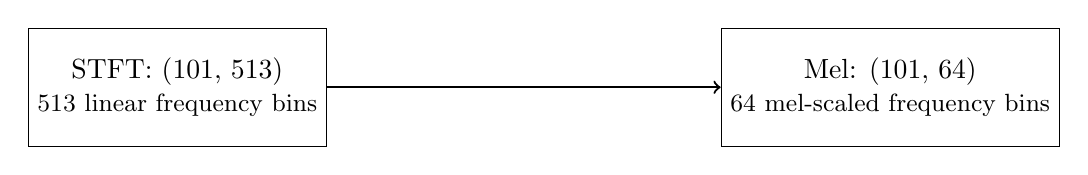
\begin{tikzpicture}[
    node distance=5cm,
    box/.style={rectangle, draw, minimum width=3.5cm, minimum height=1.5cm, align=center},
    arrow/.style={->, thick}
]

\node[box] (stft) {STFT: (101, 513)\\\small{513 linear frequency bins}};
\node[box, right=of stft] (mel) {Mel: (101, 64)\\\small{64 mel-scaled frequency bins}};

\draw[arrow] (stft) -- (mel);

\end{tikzpicture}
\end{center}

\subsection{Why This Two-Step Process?}
\begin{itemize}
    \item \textbf{STFT}: Provides temporal resolution (when frequencies occur)
    \item \textbf{Mel}: Provides perceptual frequency compression (what frequencies matter to humans)
    \item \textbf{Result}: A compact, perceptually-relevant representation perfect for emotion recognition
\end{itemize}

\section{Configuration Parameters}

\subsection{STFT Parameters}
\begin{lstlisting}[language=Python, basicstyle=\small]
window_size = 1024    # n_fft: Size of FFT window
hop_size = 320        # Distance between consecutive windows
sample_rate = 32000   # Audio sample rate
\end{lstlisting}

\subsection{Mel Parameters}
\begin{lstlisting}[language=Python, basicstyle=\small]
mel_bins = 64         # Number of mel frequency bands
fmin = 50             # Minimum frequency (Hz)
fmax = 14000          # Maximum frequency (Hz)
\end{lstlisting}

\section{Result for Machine Learning}

The final mel-spectrogram shape \textbf{(101, 64)} provides:
\begin{itemize}
    \item \textbf{101 time steps}: Temporal resolution for capturing changes over time
    \item \textbf{64 mel bins}: Perceptually-relevant frequency representation
    \item \textbf{2D image-like format}: Perfect for CNN processing
    \item \textbf{Compact representation}: Efficient for training and inference
\end{itemize}

This representation allows the model to learn both \textbf{what} sounds occur and \textbf{when} they occur, making it ideal for emotion recognition in audio.

\end{document} 